\documentclass[11pt,oneside]{book}
\usepackage[margin=1.2in]{geometry}
\usepackage[toc,page]{appendix}
\usepackage{graphicx}
\usepackage{lipsum}
\usepackage{caption}

% Added packages
\usepackage[british,UKenglish,USenglish,english,american]{babel}
\usepackage{float}
\usepackage{subfig}
\usepackage[hidelinks]{hyperref}
\usepackage[backend=bibtex,style=numeric-comp,hyperref,backref,sorting=none]{biblatex}
\addbibresource{bibliography.bib}
\usepackage{tabularx} 
\usepackage{ltxtable} 


\hypersetup{
	colorlinks   = true, %Colours links instead of ugly boxes
	urlcolor     = blue, %Colour for external hyperlinks
	linkcolor    = blue, %Colour of internal links
	citecolor   = red %Colour of citations
}
\renewcommand*{\arraystretch}{1.5}
\renewcommand\thesection{\arabic{section}}

\begin{document}
	
	\captionsetup[figure]{margin=1.5cm,font=small,labelfont={bf},name={Figure},labelsep=colon,textfont={it}}
	\captionsetup[table]{margin=1.5cm,font=small,labelfont={bf},name={Table},labelsep=colon,textfont={it}}
	\setlipsumdefault{1}
	
	\frontmatter
	
	\begin{titlepage}
		
		
		% -------------------------------------------------------------------
		% Front page
		% -------------------------------------------------------------------
		
		\begin{center}
			{\LARGE University of Padua}\\[1cm]
			{\Large Department of Computer Science}\\[2cm]
			
\includegraphics[width=5cm]{images/logo-unipd.png}\\[2cm]
			\linespread{1.2}\huge {\bfseries Skin cancer classification using Keras}\\[1.5cm]
			\linespread{1}
			{\Large Alberto Bezzon 1211016 \\ Tommaso Carraro 1210937}\\[1cm]
			%{\large \emph{Supervisor:} Supervisor's Name}\\[1cm] % if applicable
			\large The report resumes briefly the cognitive services project\\[0.5cm] 
			Academic year 2018 - 2019
		\end{center}
		
	\end{titlepage}
	
	
	% -------------------------------------------------------------------
	% Abstract
	% -------------------------------------------------------------------
	
	%\chapter*{Abstract}
briefly describe your problem, approach, and key results (no more than 300 words) 

In this paper we tried to bring the power of CNNs in skin lesions classification. We built a simple CNN model from scratch and we trained it on the popular HAM10000 dataset. We then increased its performances using common machine learning techniques, such as class weighting and data oversampling, to deal with the problem of imbalanced data. We obtained good results and we believe that in the future CNNs will be able to outperforms and probably replace expert dermatologists. In fact, it will be sufficient to provide big quantities of high quality dermoscopitic images to obtain significant results that could be used to increase the survival rate for malignant tumors.


	
	
	% -------------------------------------------------------------------
	% Contents, list of figures, list of tables
	% -------------------------------------------------------------------
	
	%\tableofcontents
	%\listoffigures
	%\listoftables
	
	
	% -------------------------------------------------------------------
	% Main sections (as required)
	% -------------------------------------------------------------------
	
	\mainmatter
	
	\section{Introduction} \label{introduction}

	Skin cancer is the most widespread cancer and one of the most dangerous because of the number of cases that not only exceeds the combined total of new cases for prostate cancer, breast cancer, lung cancer, and colorectal cancer, but also it increases from year to year. In particular, malignant melanoma is a prevalent type of cancer that is especially deadly. It is well known that early detection and proper treatments for new malignant skin cancer cases are very important to ensure high survival rate. Indeed, with an appropriate treatment in an early stage, survival rates are very promising. Otherwise, the survival rate for melanoma decreases from 99\% to 14\% in more advanced stages.
	
	\smallskip
	
	Usually, the way to detect a melanoma is by inspecting the visual details of skin, but it has a low precision. Another way is dermoscopy, a non-invasive technique that can capture a high resolution image of the skin which enables dermatologists to detect features that are invisible to the naked eye. This technique makes easier to diagnose melanoma, but it is time consuming and it is based on the clinician skills. Moreover, because of the resemblance between malignant skin tumors and benign skin lesions in visual features, it is very hard for dermatologists to differentiate between them.
	
	\smallskip
	
	In recent years, deep learning, and specifically convolutional neural networks (CNNs), have reached very good performances in skin cancer classification tasks and have allowed computers to outperform dermatologists. For this reason, in our project we have tried to improve the accuracy of skin cancer detection using state-of-the-art CNN models and techniques. In particular, we have used these models to distinguish between seven common types of skin cancers that are included in the HAM10000, a popular and recent dataset made for this specific task. We obtained the best performances on the test set using class weighting technique to train a simple CNN model built from scratch. 
	
	\bigskip
	
	This document is organized as follows:  
	\begin{itemize}
		\item Section \ref{related_works} presents related works for ``Skin cancer classification'';
		\item Section \ref{dataset} provides the description of dataset used in our experiments;
		\item Section \ref{proposed_model} includes the approach we used for solving the problem;
		\item Section \ref{experiments} presents the experiments we made on the proposed model;
		\item Section \ref{conclusion} contains the conclusion and future works.
	\end{itemize}
	\section{Related works} \label{related_works}

	We have viewed different state-of-the-art papers. 
	In \cite{article1}, researchers used Google’s Inception v3 CNN architecture pretrained on the 2014 ImageNet Challenge. They then removed the final classification layer from the network and retrained it with their dataset, fine-tuning the parameters across all layers. During training they resized each image to 299 x 299 pixels in order to made it compatible with the original dimensions of the Inception v3 network architecture. All layers of the network were fine-tuned using the same global learning rate and RMSProp optimizer. They performed their experiments on a 129.000 images dataset, created from a combination of different datasets. They obtained 72.1\% overall accuracy training their model on 757 classes. To create these training classes they used a taxonomy of skin disease and a partitioning algorithm that maps diseases into training classes. We have tried to obtain these data, but they were protected by the Stanford Hospital.
	
	\smallskip
	
	In \cite{article3}, researchers studied the effectiveness and capability of different pre-trained state-of-the-art CNNs architectures (DenseNet 201, ResNet 152, Inception v3, InceptionResNet v2). All the models they used were pre-trained on the 2014 ImageNet Challenge. They changed the classification part of these models with a custom classifier and they retrained them across all the layers using different hyperparameters depending on the specific network architecture. They trained these models on a dataset composed of 10.135 dermoscopy skin images composed by the combination of HAM10000 and PH2 datasets.  The aim of their project was to compare the ability of deep learning with the performances of highly trained dermatologists. Overall, the mean results show that all deep learning models outperformed dermatologists (at least 11\%). The best ROC AUC values for melanoma and basal cell carcinoma are 94.40\% (ResNet 152) and 99.30\% (DenseNet 201) versus 82.26\% and 88.82\% of dermatologists, respectively.
	
	\smallskip

	In \cite{article2}, researchers used a CNN model built from scratch. The proposed model architecture consists on a sequence of alternating Conv2D and MaxPooling2D layers that form the core building blocks of modern CNNs. Then, they putted a batch normalization layer after each ReLu activation. They used this model to perform a binary classification task, in fact the first convolutional layer takes in 224 x 224 skin lesion images and the last dense layer contains a single unit with sigmoid activation in order to output the resulting classes (benign and malignant). They trained their model on the PHDB melanoma dataset, created by their own from a combination of open access datasets. They obtained an accuracy of the 86\% on this dataset and regularization techniques such as dropout and data augmentation techniques were heavily relied upon to combat the overfitting problem.
	
	\smallskip
	
	After reading these papers we decided firstly to try the power of transfer learning on our dataset. Given the big amount of data in HAM10000 and the high difference between the images in our dataset and the images included in the ImageNet Challenge, the best transfer learning strategy was to train the pre-trained model across all the layers, but we did not have enough resources for it. So, we froze all the layers except for the classification part of the network and we trained the model. This technique gave us bad performances compare to the training of a simple CNN model built from scratch. So, we decided to use an approach that is more similar to the method explained in \cite{article2} than the other papers.
	
	\section{Dataset} \label{dataset}

	On the Internet there are few open access datasets for skin cancer classification task, and most of them contain a collection of bad quality images that are not biopsy proven. We read a lot of papers on this task and in most of them researchers had to create a dataset from scratch for the unavailability of a complete dataset composed of quality and biopsy proven images on the web. In most cases they took best images from different sources and they built their own dataset. Recently, some researchers and dermatologists understood the importance of this task and decided to create a new dataset, called HAM10000, that we used on our project. 
	This dataset contains 10015 dermatoscopic images that were collected over a period of 20 years from two different sites: the Department of Dermatology at the Medical University of Vienna, Austria, and the skin cancer practice of Cliff Rosendahl in Queensland, Australia. It includes pigmented lesions from different populations. The Austrian image set consists of lesions of patients referred to a tertiary European referral center specialized for early detection of melanoma in high risk groups. The Australian image set includes lesions from patients of a primary care facility in a high skin cancer incidence area. Dermatoscopic images of both study sites were taken by different devices using polarized and non-polarized dermatoscopy. The set includes representative examples of pigmented skin lesions that are practically relevant. More than 95\% of all lesion encountered during clinical practice will fall into one of the seven diagnostic categories contained in the dataset. In practice, the task of the clinician is to differentiate between malignant and benign lesions, but also to make specific diagnoses because different malignant lesions may be treated in a different way and timeframe. The number of images in the dataset does not correspond to the number of unique lesions, because experts also provided images of the same lesion taken at different magnifications or angles, or with different cameras. This should serve as a natural data-augmentation as it shows random transformations and visualizes both general and local features.
	
	\bigskip
	
	The seven different skin lesions categories contained in the dataset are:
	
	\paragraph{akiec}
	Actinic Keratoses (Solar Keratoses) and Intraepithelial Carcinoma (Bowen's disease) are common non-invasive, variants of squamous cell carcinoma that can be treated locally without surgery. There is agreement that these lesions may progress to invasive squamous cell carcinoma. 
	
	\paragraph{bcc}
	Basal cell carcinoma is a common variant of epithelial skin cancer that rarely metastasizes but grows destructively if untreated. 
	
	\paragraph{bkl}
	``Benign keratosis" is a generic class that includes seborrheic keratoses (``senile wart"), solar lentigo and lichen-planus like keratoses (LPLK), which corresponds to a seborrheic keratosis or a solar lentigo with inflammation and regression. From a dermatoscopic view, lichen planus-like keratoses are especially challenging because they can show morphologic features mimicking melanoma and are often biopsied or excised for diagnostic reasons. 
	
	\paragraph{df}
	Dermatofibroma is a benign skin lesion regarded as either a benign proliferation or an inflammatory reaction to minimal trauma. 
	
	\paragraph{nv}
	Melanocytic nevi are benign neoplasms of melanocytes and appear in a myriad of variants, which all are included in this dataset. The variants may differ significantly from a dermatoscopic point of view.
	
	\paragraph{mel}
	Melanoma is a malignant neoplasm derived from melanocytes that may appear in different variants. If excised in an early stage it can be cured by simple surgical excision. 
	
	\paragraph{vasc}
	Vascular skin lesions in the dataset range from cherry angiomas to angiokeratomas and pyogenic granulomas. Hemorrhage is also included in this category.
	
	\bigskip
	
	In Figure \ref{fig:category_samples} is possible to see the differences between these types of skin lesions.
	
	\begin{figure}[H]
		\centering
		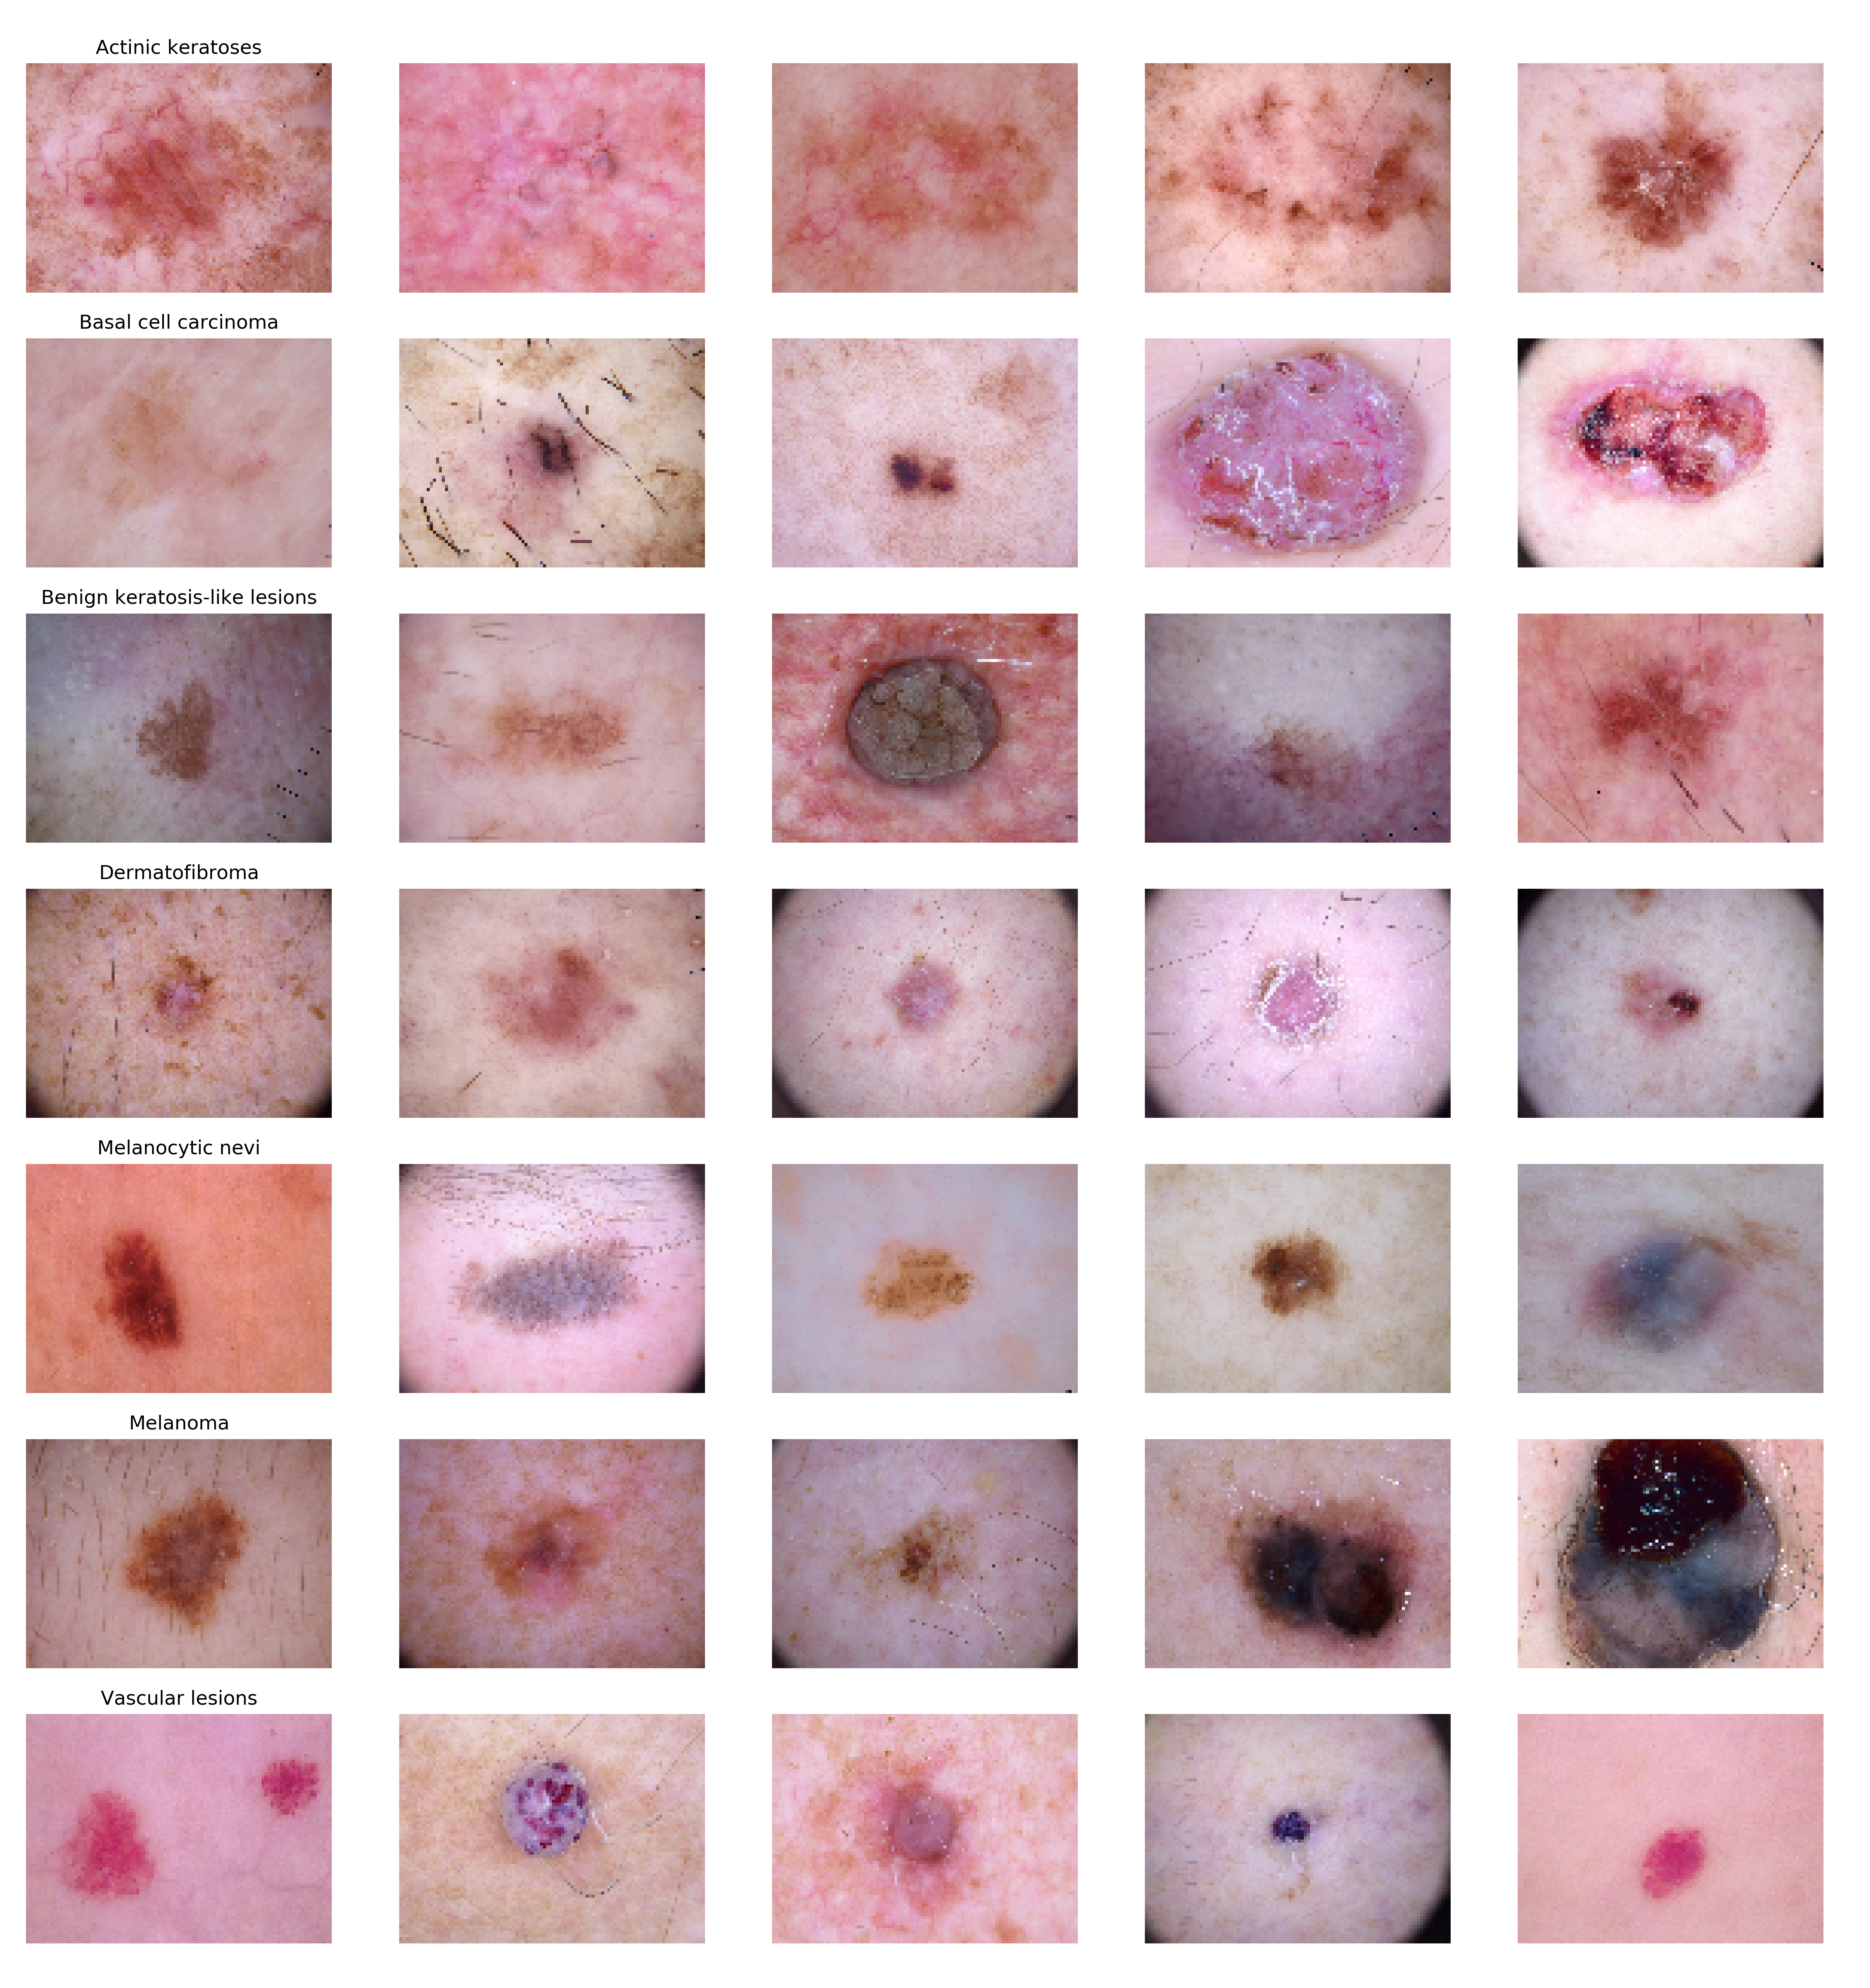
\includegraphics[width=15cm]{images/category_samples.png}
		\caption{Skin lesions categories in HAM10000}
		\label{fig:category_samples}
	\end{figure}
	
	Imbalanced data is the biggest problem of HAM10000, in fact Melanocytic nevi is the majority class with 67\% of examples, instead Dermatofibroma is the minority class with only 4\% of examples. In Figure \ref{fig:graph1} is possible to see the distribution of these skin lesions HAM10000. 
	
	\smallskip
	
	Imbalanced data is a common issue of skin cancer datasets and have been a challenge for this project. Initially we thought to find other images to oversample the dataset, but then we turned out that images in the Internet are bad in quality and different compared to the images of the HAM10000, so we have decided to keep it at the original version.
	Data preprocessing in this dataset has been limited to the normalization of images and the transformation of labels in one-hot encoded vectors to make the network capable to learn from them. We have decided to split the dataset in 80\% training set and 10\% test set, then we took a 10\% validation set from the training set. We kept this aggressive split because of the limited amount of data, in fact we want our model to learn as much as possible features from the dataset. Images have been resized to 100x75 before being supplied to the CNN model. We have decided this specific size because experiments showed that our model works better with small resolution images.
	
	\begin{figure}[H]
		\centering
		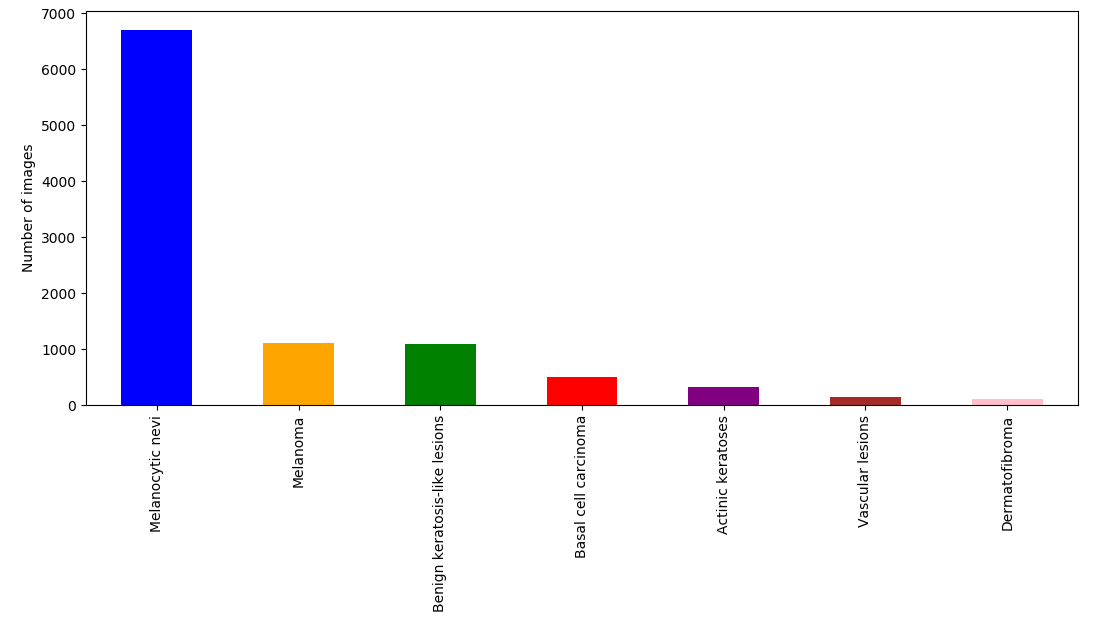
\includegraphics[width=15cm]{images/graph1.png}
		\caption{Distribution of skin lesions categories in HAM10000}
		\label{fig:graph1}
	\end{figure}
	\section{Proposed model} \label{proposed_model}

	\subsection{Performance measures choice}
		
		As mentioned in Section \ref{dataset} HAM10000 is a highly imbalanced dataset and it has been a challenge to deal with it. The first problem we faced was on the choice of the right performance measure for our experiments. Accuracy is usually referred as the best performance measure for image classification tasks but in case of imbalanced data is definitely not the right choice. In fact, if the accuracy is high it does not mean that we have found a good model, because it can be possible that it is high only because our model is very good in predicting majority classes, but we want our model to be accurate on all the classes, even the most challenging minority classes.
		
		\smallskip
		
		Our goal is to obtain a model that maximize both precision and recall on all the classes.
		To achieve this goal, we have decided to use F1-measure and macro average performance measures. F1-measure allows to understand in which classes our model performs well: a high F1 score for one class means that our model returns a high precision but also a high recall on that specific class. 
		
		\smallskip
		
		We have then selected the macro average F1 because we are interested in knowing if our model performs well in minority classes, which include malign skin cancers, such as melanoma class, that is the most important one in the dataset. 
		Moreover, if the model performs well in minority classes, even if the number of examples is limited, means that it is able to learn the correct features to discriminate between these classes. 
		
		\smallskip
		
		Finally, since we are interested in predicting well malign skin cancers, we did not use micro average because it returns high scores when the model performs well in majority classes, which include benign tumors.
		
	\subsection{Transfer learning attempt}
		
		As mentioned in Section \ref{related_works} we firstly tried to apply transfer learning on our task. We took Inception v3 model, pre-trained on ImageNet Challenge, and we then changed the classification part on top of it with a custom classifier. This classifier was composed of one global average pooling layer, two fully connected layers and finally a softmax layer. We took this architecture from \cite{article2} because they had obtained the best results we have found on HAM10000. We froze all the layers except of the custom classification part and we trained our model with the settings reported in \cite{article2}. We obtained bad performances with this model compared to the performance reported in the paper. The accuracy was relatively high (67\%) but when we moved to the confusion matrix we discovered that the model was predicting everything like a Melanocytic Nevi to maximize the overall accuracy. So, the model wasn't able to learn anything. After this test we decided to move to the classic CNN architecture, in fact transfer learning performs well when the dataset is similar to the ImageNet dataset and it wasn't the case.
		
	\subsection{Architecture of proposed model}
	
		For the design of our CNN model architecture we have followed a common design pattern in CNN. This pattern consists in building a simple model architecture with only one convolutional block and to increase its depth until the adding of a new convolutional block does not give better performance compared to the last model built. We proceeded this way because we found that this pattern performs well in general image classification tasks and the experiments in \cite{article3} showed that it performs well even in skin cancer classification task. So, we began our project with the construction of a base model that we have then tried to improve. In Figure \ref{fig:base_model} we present our base model. Its architecture is composed of a convolutional block and a simple classification block, which are the building blocks of modern CNN architectures. The convolutional block is composed of two convolutional layers with 32 activation maps followed by a max pooling layer. We have decided to set a 3x3 filter size for the convolutional layers because local features in skin lesions are relatively small. The classification block is composed of a flatten layer used to flat the output of the convolutional block, a fully connected layer with 64 units and finally a softmax layer. We have then added a dropout layer after the fully connected layer. We will explain our regularizations techniques in section (regularization). 
		
		\begin{figure}[H]
			\centering
			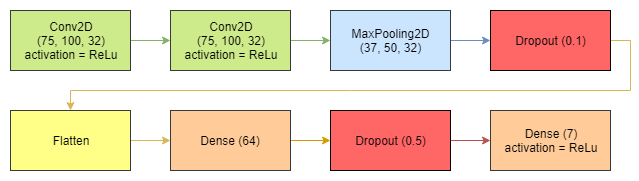
\includegraphics[width=15cm]{images/base_model.png}
			\caption{Base model architecture}
			\label{fig:base_model}
		\end{figure}
	
		Given the base model we began to add convolutional blocks to it to see if model performances increased. The adding of a convolutional block consists in add two convolutional layers with doubled activation maps followed by a max pooling layer after the previous convolutional block of the net. With this technique we have changed the architecture of our base model five times until we obtained our best and proposed model. In Table \ref{tab:models_performances} is possible to compare the performances of the models we have tried. The table presents the F1 scores for all the classes, the macro average of the f1 score and the test accuracy for each model. We trained these models with the settings reported in Section \ref{training_settings}.
		
		\begin{table}[H]
			\small
			\begin{threeparttable}
				\begin{tabular}{ |>{\centering\arraybackslash}p{2cm}|c|c|c|c|c|c|c|>{\centering\arraybackslash}p{2cm}|>{\centering\arraybackslash}p{2cm}| }
					\hline
					\textbf{Model} & \textbf{akiec} & \textbf{bcc} & \textbf{bkl} & \textbf{df} & \textbf{mel} & \textbf{nv} & \textbf{vasc} & \textbf{Macro average} & \textbf{Test accuracy} \\ \hline
					
					Base model\tnotex{tnote:model1} & 0.32 & 0.45 & 0.47 & 0.13 & 0.34 & 0.87 & 0.49 & 0.44 & 0.74 \\ \hline
					Model 2\tnotex{tnote:model2} & 0.40 & 0.53 & 0.50 & 0.00 & 0.36 & 0.88 & 0.72 & 0.48 & 0.76 \\ \hline
					Model 3\tnotex{tnote:model3} & 0.38 & 0.52 & 0.52 & 0.07 & 0.47 & 0.89 & 0.58 & 0.49 & 0.77 \\ \hline
					Proposed model\tnotex{tnote:model4} & 0.41 & 0.52 & 0.53 & 0.16 & 0.38 & 0.90 & 0.65 & 0.51 & 0.76 \\ \hline
					Model 5\tnotex{tnote:model5} & 0.34 & 0.46 & 0.53 & 0.07 & 0.39 & 0.90 & 0.62 & 0.47 & 0.75 \\ \hline
					
				\end{tabular}		
				\begin{tablenotes}
					\item\label{tnote:model1} $2 x Conv2D(32) \rightarrow MaxPool2D \rightarrow Flatten \rightarrow FC(64) \rightarrow Dropout(0.5) \rightarrow Softmax(7)$
					\item\label{tnote:model2} $2 x Conv2D(32) \rightarrow MaxPool2D \rightarrow 2 x Conv2D(64) \rightarrow MaxPool2D \rightarrow Flatten \rightarrow FC(128) \rightarrow Dropout(0.5) \rightarrow Softmax(7)$
					\item\label{tnote:model3} $2 x Conv2D(32) \rightarrow MaxPool2D \rightarrow 2 x Conv2D(64) \rightarrow MaxPool2D \rightarrow 2 x Conv2D(128) \rightarrow MaxPool2D \rightarrow Flatten \rightarrow FC(256) \rightarrow Dropout(0.5) \rightarrow Softmax(7)$
					\item\label{tnote:model4} $2 x Conv2D(32) \rightarrow MaxPool2D \rightarrow 2 x Conv2D(64) \rightarrow MaxPool2D \rightarrow 2 x Conv2D(128) \rightarrow MaxPool2D \rightarrow 2 x Conv2D(256) \rightarrow MaxPool2D \rightarrow Flatten \rightarrow FC(512) \rightarrow Dropout(0.5) \rightarrow Softmax(7)$
					\item\label{tnote:model5} $2 x Conv2D(32) \rightarrow MaxPool2D \rightarrow 2 x Conv2D(64) \rightarrow MaxPool2D \rightarrow 2 x Conv2D(128) \rightarrow MaxPool2D \rightarrow 2 x Conv2D(256) \rightarrow MaxPool2D \rightarrow 2 x Conv2D(512) \rightarrow MaxPool2D \rightarrow Flatten \rightarrow FC(1024) \rightarrow Dropout(0.5) \rightarrow Softmax(7)$
				\end{tablenotes}
			\end{threeparttable}
			\caption{Models performances}
			\label{tab:models_performances}
		\end{table}
	
		The base model has the worst performances compared to the other models. Model 2 increases the performances of the base model on all the classes, but it has the problem to be bad in classifying Dermatofibromas.
		Model 3 has the best accuracy on the test set but a macro average that is less than our proposed model and we prefer to balance the number of correct classifications over the classes instead of increasing the overall accuracy. 
		Even if model 3 has the best performance on melanoma detection we chose model 4 because we think it is able to capture more complex features on the images, in fact it has the highest F1 score in Dermatofibroma class, that seems to be the most difficult to classify for our models, and also it outperforms the other models on all the other classes. We think that our proposed model can reached these performances thanks to the number of convolutional blocks on it, in fact more convolutional blocks a network has and more complex features on the images will be able to detect. Moreover, we observed that model 4 has reached the maximum depth for our CNN in this specific task, in fact the adding of another convolutional block decreases most of the metrics scores.
		Finally, every time we added a new convolutional block we doubled also the number of units in the fully connected layer at the top of the network. We chose this strategy because more complex are the features that the convolution block is able to identify and more units in the fully connected layer will be required to capture these complex features.
		
		\begin{figure}[H]
			\centering
			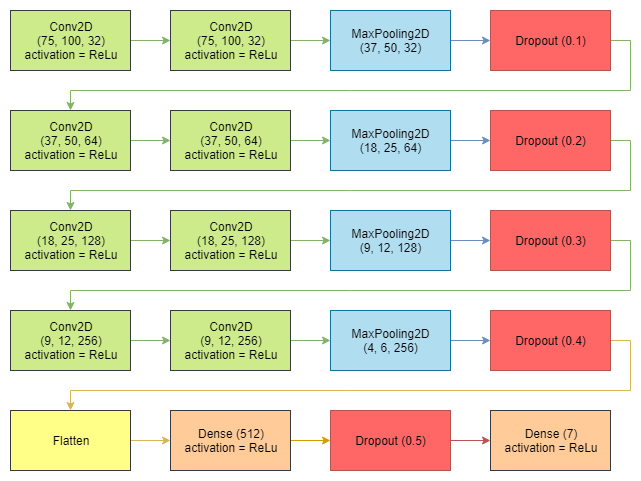
\includegraphics[width=15cm]{images/proposed_model.png}
			\caption{Proposed model architecture}
			\label{fig:proposed_model}
		\end{figure}
		
		In Figure \ref{fig:proposed_model} we present the proposed model architecture. It performs well on HAM10000 compared to transfer learning and it has the advantage of the simplicity in the architecture. It is less depth and it takes faster training times thanks to the smaller number of parameters to be learnt. 
		After we have found the best architecture for this task we tried to do some experiments to increase its performances, such as class weighting and oversampling with data augmentation to deal with the problem of imbalanced data. In Section \ref{experiments} we present these experiments.
	
	\subsection{Regularizations and training settings}
	
		\subsubsection{Regularizations techniques} \label{regularization_techniques}
		
			To prevent overfitting in our models we decided to use three common regularizations techniques:
			
			\begin{itemize}
				\item \textbf{Dropout layers:} in previous section we presented our model architecture and it presents five dropout layers. The dropout layer after the fully connected layer freezes half of the units at each epoch. We set this percentage because it is well known that fully connected layers are highly subject to overfitting. We then decided to add a dropout layer after each convolutional block, with an increasing percentage of frozen units. Since the number of parameters to be learnt increases with the increase of the depth of the network this configuration helped our network to mitigate the overfitting issue;
				\item \textbf{Learning rate decay:} we set our model to decay the learning rate if no improvements on the validation accuracy are showed after 3 epochs of training. We tried many experiments and we discovered that this configuration helped the network avoids overfitting;
				\item \textbf{Early stopping:} since dropout and learning rate decay were not enough to avoid overfitting, early stopping was the next choice. Our models are configured to stop the learning in case of high overfitting. If the validation accuracy does not increase in 10 epochs, the training will be stopped and the weights corresponding to the best validation accuracy will be restored. We decided this configuration because we observed that in many cases the model needed many epochs to continue to learn.
			\end{itemize}
		
		\subsubsection{Optimizer and optimizer hyperparameters choice}
			
			We have tried three optimizers for the gradient descent: Stochastic Gradient Descent, RMSprop and Adam optimizers. We limited the test to these three optimizers because we found they are commonly used in skin classification tasks. SGD and RMSprop did not perform well on our task. They did not allow the net to train, in fact the validation accuracy was stuck at 68\%. We had the same problem of transfer learning. We then tried Adam optimizer and the network began to learn.
			
			\smallskip
			
			We have selected only the learning rate of the Adam optimizer and we left all the other parameters at their default. We tried to train our models with a 0.001 learning rate. We have found that is the common choice in computer vision, but in our case the learning was too fast and the network began to overfit soon. We tried 0.00001 learning rate and we observed that the convergence was very stable, in fact the training accuracy and the validation accuracy followed the same behavior, but models took too much epochs to converge and very often the early stopping stopped the training even if there was not overfitting because 10 epochs were not enough to improve the training accuracy.
			
			\smallskip
			
			Finally, we have selected 0.0001 learning rate because we observed it was the best tradeoff between convergence speed and overfitting.
			In Figure \ref{fig:val_acc_lr} we show how training and validation accuracy behaviours change with the change of the learning rate.
			
			\begin{figure}[!h] 
				\subfloat[Learning rate 0.001]{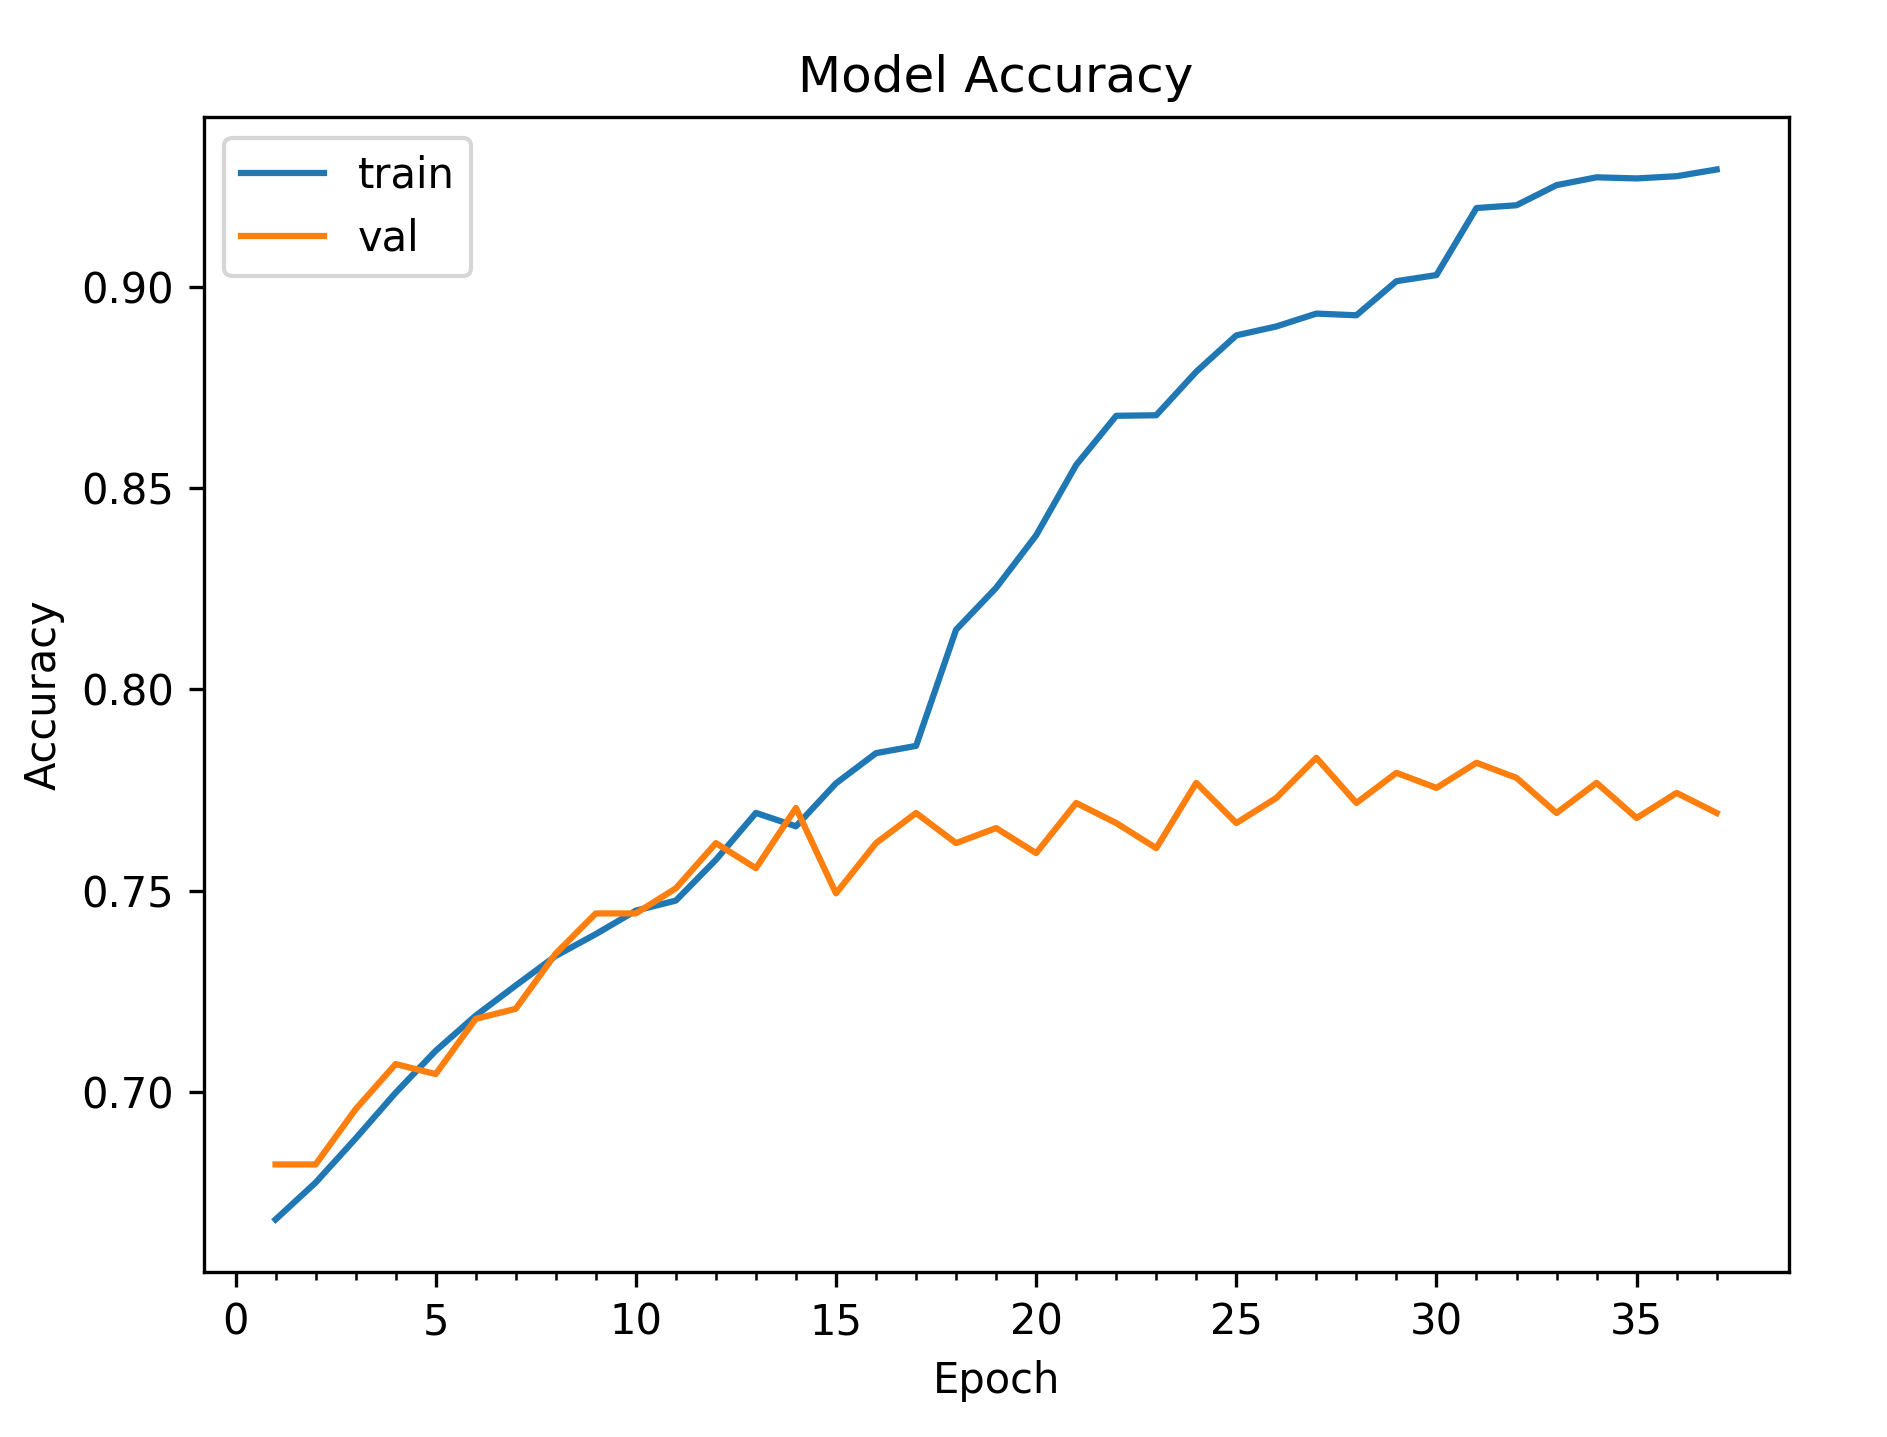
\includegraphics[width=0.33\columnwidth]{images/accuracy-loss-001.png}}
				\hspace*{\fill}
				\subfloat[Learning rate 0.00001]{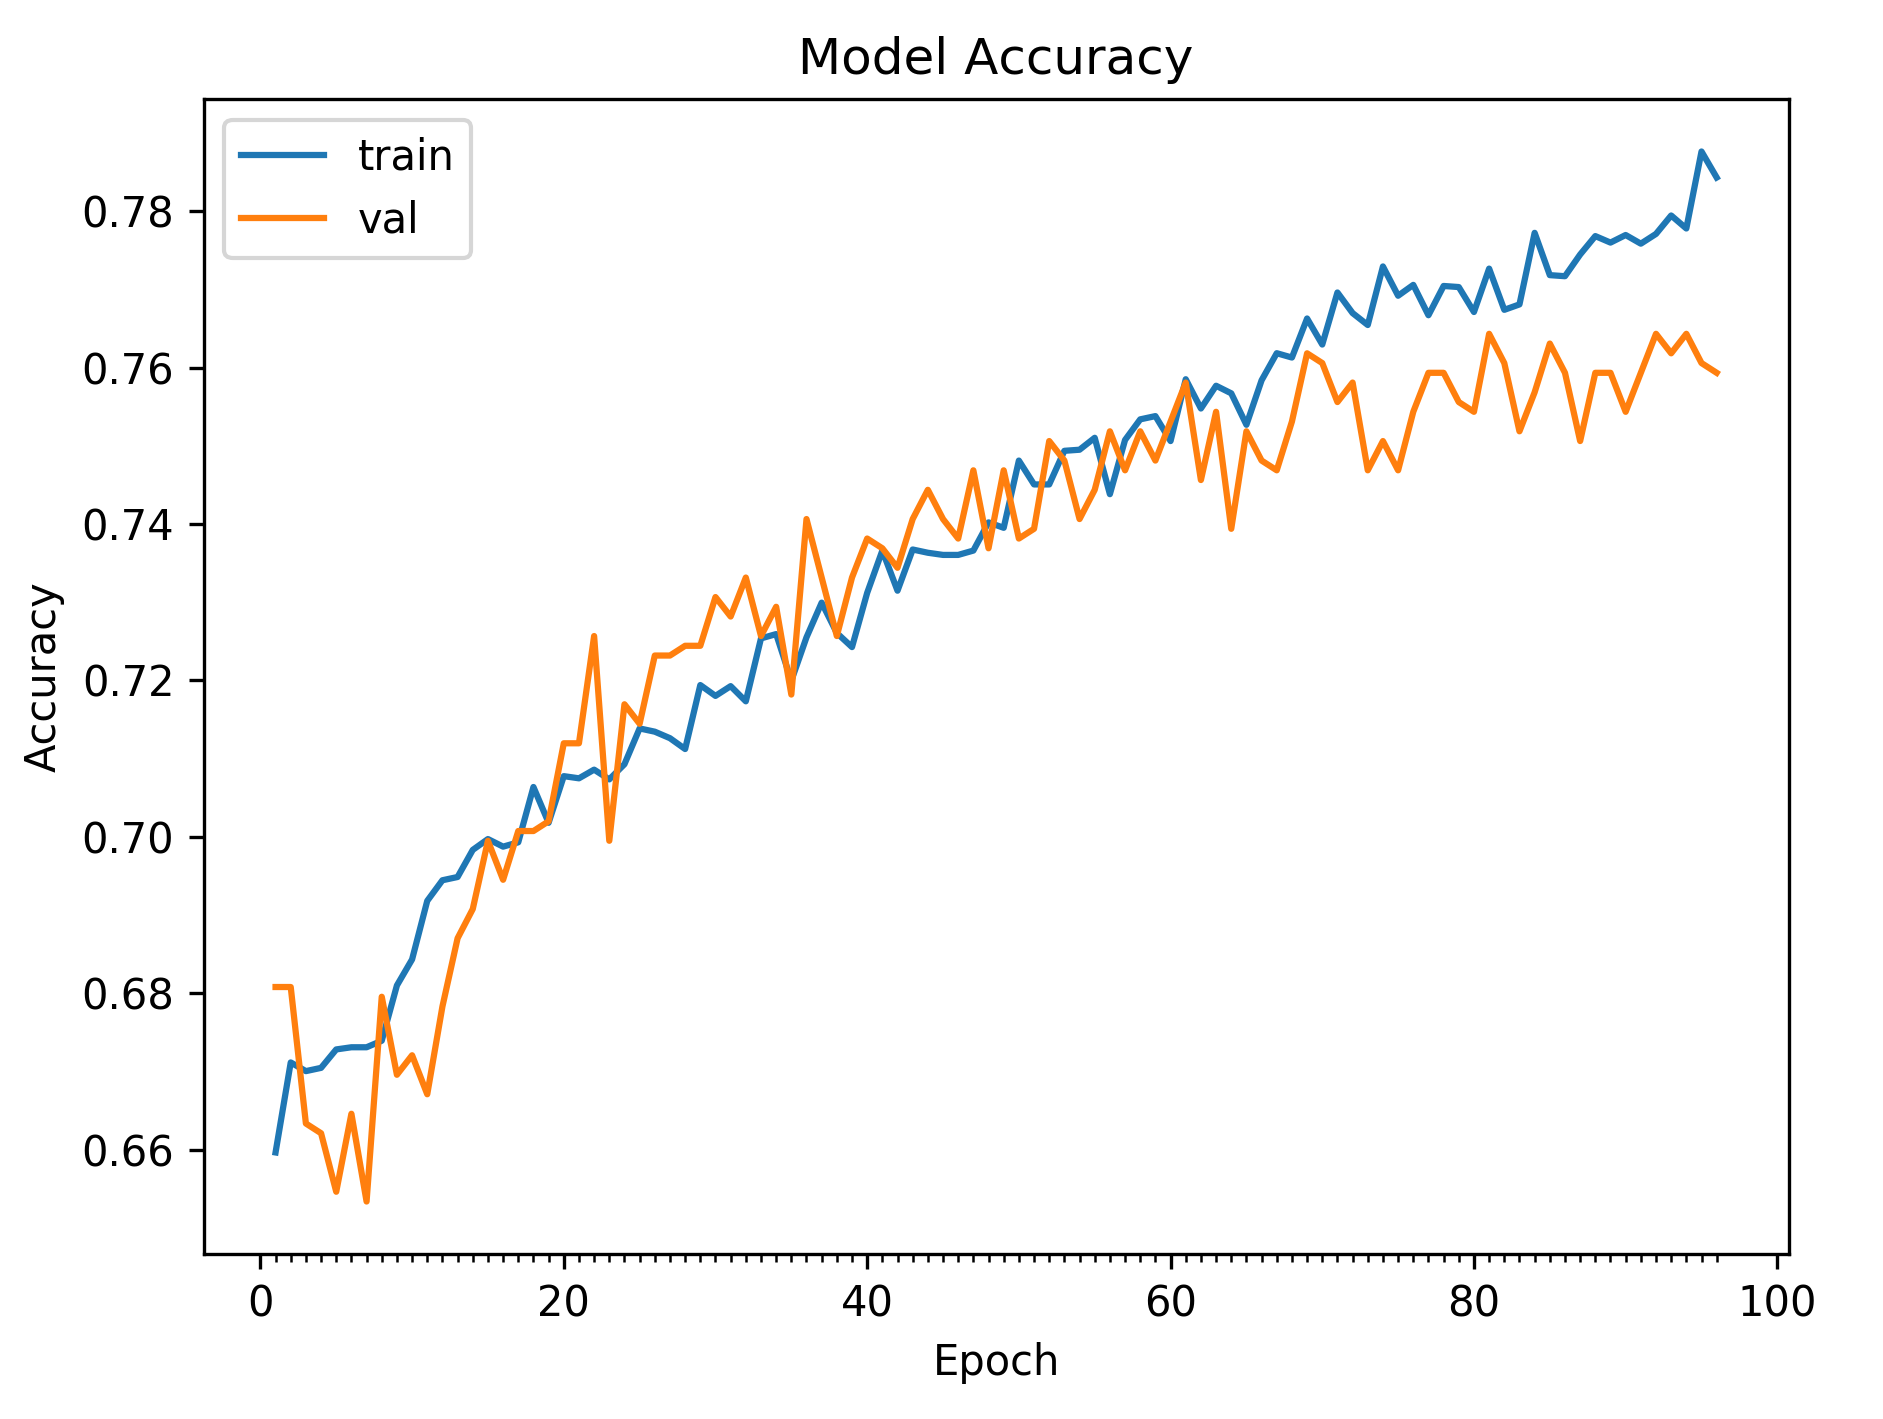
\includegraphics[width=0.33\columnwidth]{images/accuracy-loss-00001.png}}
				\hspace*{\fill}
				\subfloat[Learning rate 0.0001]{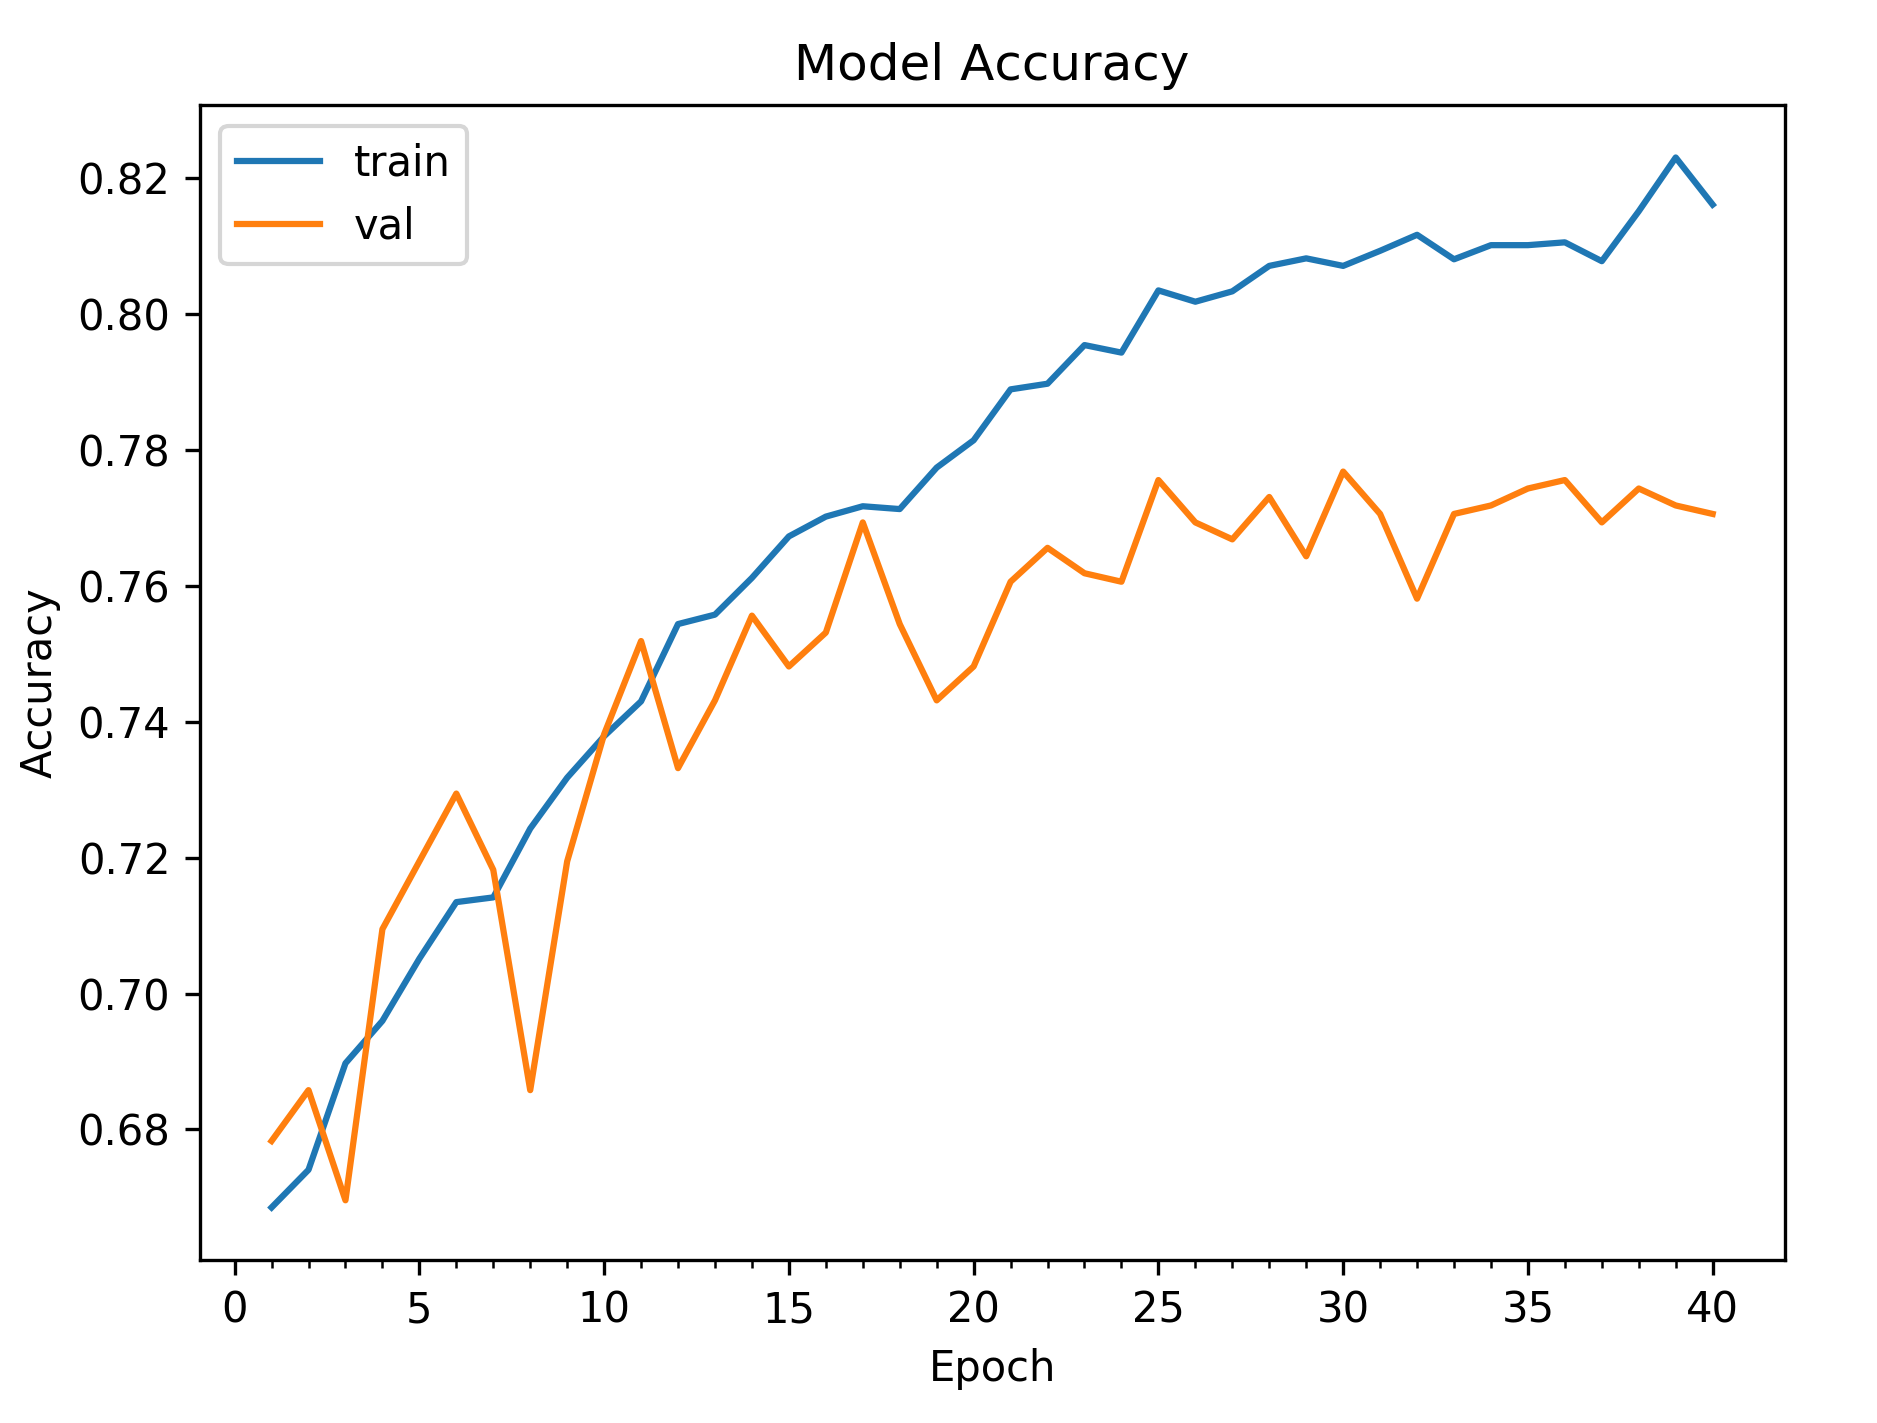
\includegraphics[width=0.33\columnwidth]{images/accuracy-loss-0001.png}}
				\caption{Validation accuracy plot with different learning rate}
				\label{fig:val_acc_lr}
			\end{figure}
			
		\subsubsection{Training settings} \label{training_settings}
		
			We have trained all our models with these settings:
			\begin{itemize}
				\item Adam optimizer with 0.0001 learning rate and the other optimizer parameters at their default;
				\item categorical cross entropy loss function;
				\item 32 batch size: this is the default batch size in keras and we observed good performances on our model with this batch size;
				\item 200 epochs: we decided this number to allow the network to learn as much as possible from the training set. If the model begins to overfit the early stopping will stop the training and it will restore the best weights;
				\item Regularization techniques showed in section \ref{regularization_techniques}.
			\end{itemize}	
			
			
		
		
		
		
		
		
		
	\section{Experiments} \label{experiments}

	\subsection{Experimental enviroments}
	
		Training a deep learning model that involves intensive compute tasks on large dataset can take days to run on a single CPU or a slow GPU. In our case, since HAM10000 dataset has 10015 images, it is unthinkable to perform the training of a convolutional neural network with a standard laptop. The solution turned to cloud computing. The choice fells on Google Cloud Platform because of the availability of free tier that consists in 300\$ free credits that can be used in any GCP product. 
		
		\smallskip
		
		We have tested our CNN models on a custom instance of Compute Engine. Our VM’s configuration is presented in Table \ref{tab:hw-config}
		
		\begin{table}[H]
			\centering
			\begin{tabular}{ |c|c|c|c|c|c| }
				\hline
				\textbf{Operating System} & \textbf{CPU} & \textbf{Memory} & \textbf{Disk} & \textbf{GPU} \\ \hline
				
				Ubuntu 18.04 LTS & 8 core & 52 GB & SSD / 100 GB & 1x NVIDIA Tesla K80 \\ \hline
				
			\end{tabular}
			\caption{Virtual machine configuration}
			\label{tab:hw-config}
		\end{table}
	
		Our models have been implemented in keras using tensorflow as a backend. The code is available on our GitHub repository: \url{https://github.com/albertobezzon/cognitiveservices}
		
	\subsubsection{Proposed model performances}
	
		In Figure \ref{fig:first-matrix} we show the performances of our proposed model on the test set. It is possible to see that our model has difficulties in predicting Dermatofibromas (only 11\% correctly classified) and Melanomas (only 27\% correctly classified).In particular, Dermatofibromas are confused with basal cell carcinomas (33\% of Dermatofibromas are classified like a basal cell carcinoma) and Melanocytic Nevis (33\% of Dermatofibromas are classified like a Melanocytic nevi), while Melanomas are confused with Melanocytic nevis (46\% of Melanomas are classified like a nevi). 
		This means that these classes are similar in terms of features and the imbalanced of the dataset doesn’t help in discriminating well between them. We have too few examples for Dermatofibromas and too much examples for Melanocytic Nevis. Similar problems are also present in few of the other classes.
		
		\begin{figure}[H]
			\centering
			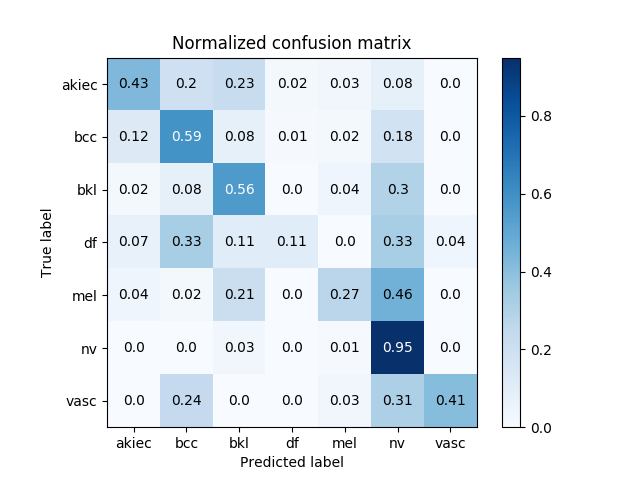
\includegraphics[width=15cm]{images/firstMatrix.png}
			\caption{Confusion matrix}
			\label{fig:first-matrix}
		\end{figure}
		
	\subsubsection{Class weighting}
	
		The first technique we tried to deal with the problem of imbalanced data is class weighting. This technique consists in assigning a weight to each class in such a way that allows to the model to give more emphasis to minority classes and less emphasis to majority classes. The idea is to assign more priority to the classes with less examples and less priority to the classes with more examples. In this way it is possible to balance the training set for the model. 
		In Figure \ref{fig:second-matrix} we show the performances of our proposed model on the test set with the class weighting technique.
		Even if the test accuracy of the model with class weighting is lower (65\% against 77\% of the previous model), it is possible to see that the correct classifications are better distributed over all the classes and this is our main goal. In fact, with class weighting the 48\% of Dermatofibromas is correctly classified and the 53\% of Melanomas. Moreover, it seems that with the class weighting our proposed model is able to distinguish better between Dermatofibromas and Melanocytic nevis, but also between Melanomas and Melanocytic nevis. Finally, it seems that also the number of misclassified examples is better distributed on the matrix. There are still difficulties in distinguishing between Dermatofibromas and Basal cell carcinoma, but we think it is possible to make the model more accurate with more training data.
		
		\begin{figure}[H]
			\centering
			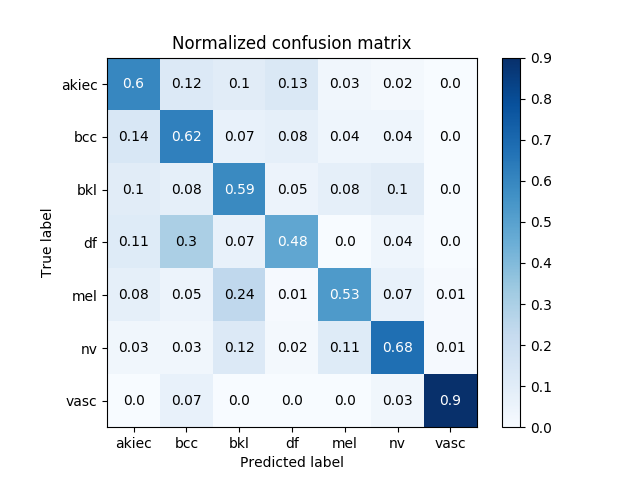
\includegraphics[width=15cm]{images/secondMatrix.png}
			\caption{Confusion matrix}
			\label{fig:second-matrix}
		\end{figure}
		
	\subsubsection{Oversampling with data augmentation}
	
		The last experiment we tried on HAM10000 is the oversampling of minority classes with data augmentation. After splitting the dataset as reported in section (dataset), the number of examples in Melanocytic nevis class was 4868, so we applied data augmentation to all the other classes to obtain a balanced training set. After applying these procedures, we obtained a 34.076 images training set.
		To oversampling the training set we have used keras’ ImageDataGenerator with the following parameters:
		\begin{itemize}
			\item rotation range: 45; 
			\item zoom range: 0.2; 
			\item width shift range: 0.1;
			\item height shift range: 0.1;
			\item horizontal flip: true; 
			\item vertical flip: true;
			\item fill mode: nearest.
		\end{itemize}
		
		After data augmentation we checked that the generated images were good and then we trained our proposed model on the augmented training set.
		In Figure \ref{fig:third-matrix} we show the performances on the test set of our proposed model with the oversampling technique.
		
		\begin{figure}[H]
			\centering
			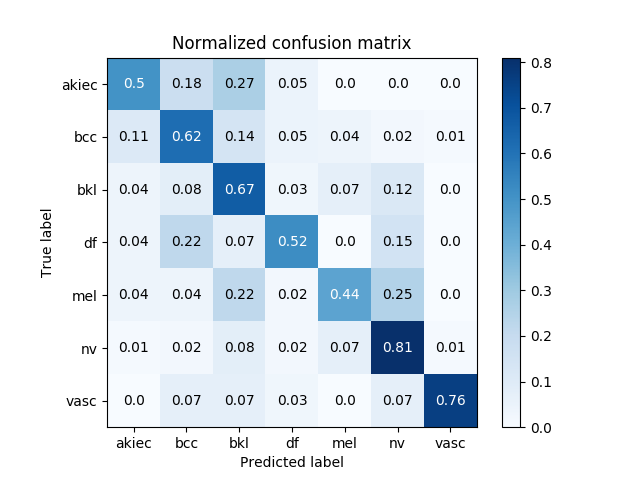
\includegraphics[width=15cm]{images/thirdMatrix.png}
			\caption{Confusion matrix}
			\label{fig:third-matrix}
		\end{figure}
		
		Unfortunately, we did not achieve the desired results, in fact even if the model trained on oversampled dataset is better in predicting Dermatofibromas (52\% well classified Dermatofibromas against 48\% of the previous model), and this explains the higher macro average f1 (0.56 against 0.51), it reintroduces difficulties in distinguish between Melanomas and Melanocytic nevis (25\% of Melanomas are classified like a Melanocytic nevi). 
		Moreover, due to aggressive data augmentation (we added more than 4000 augmented images to Dermatofibroma class) the model tends to badly overfit, even if regularizations techniques are configured. In Figure \ref{fig:overfitting-data-aug} is possible to see the overfitting of this last model.
		
		\begin{figure}[H]
			\centering
			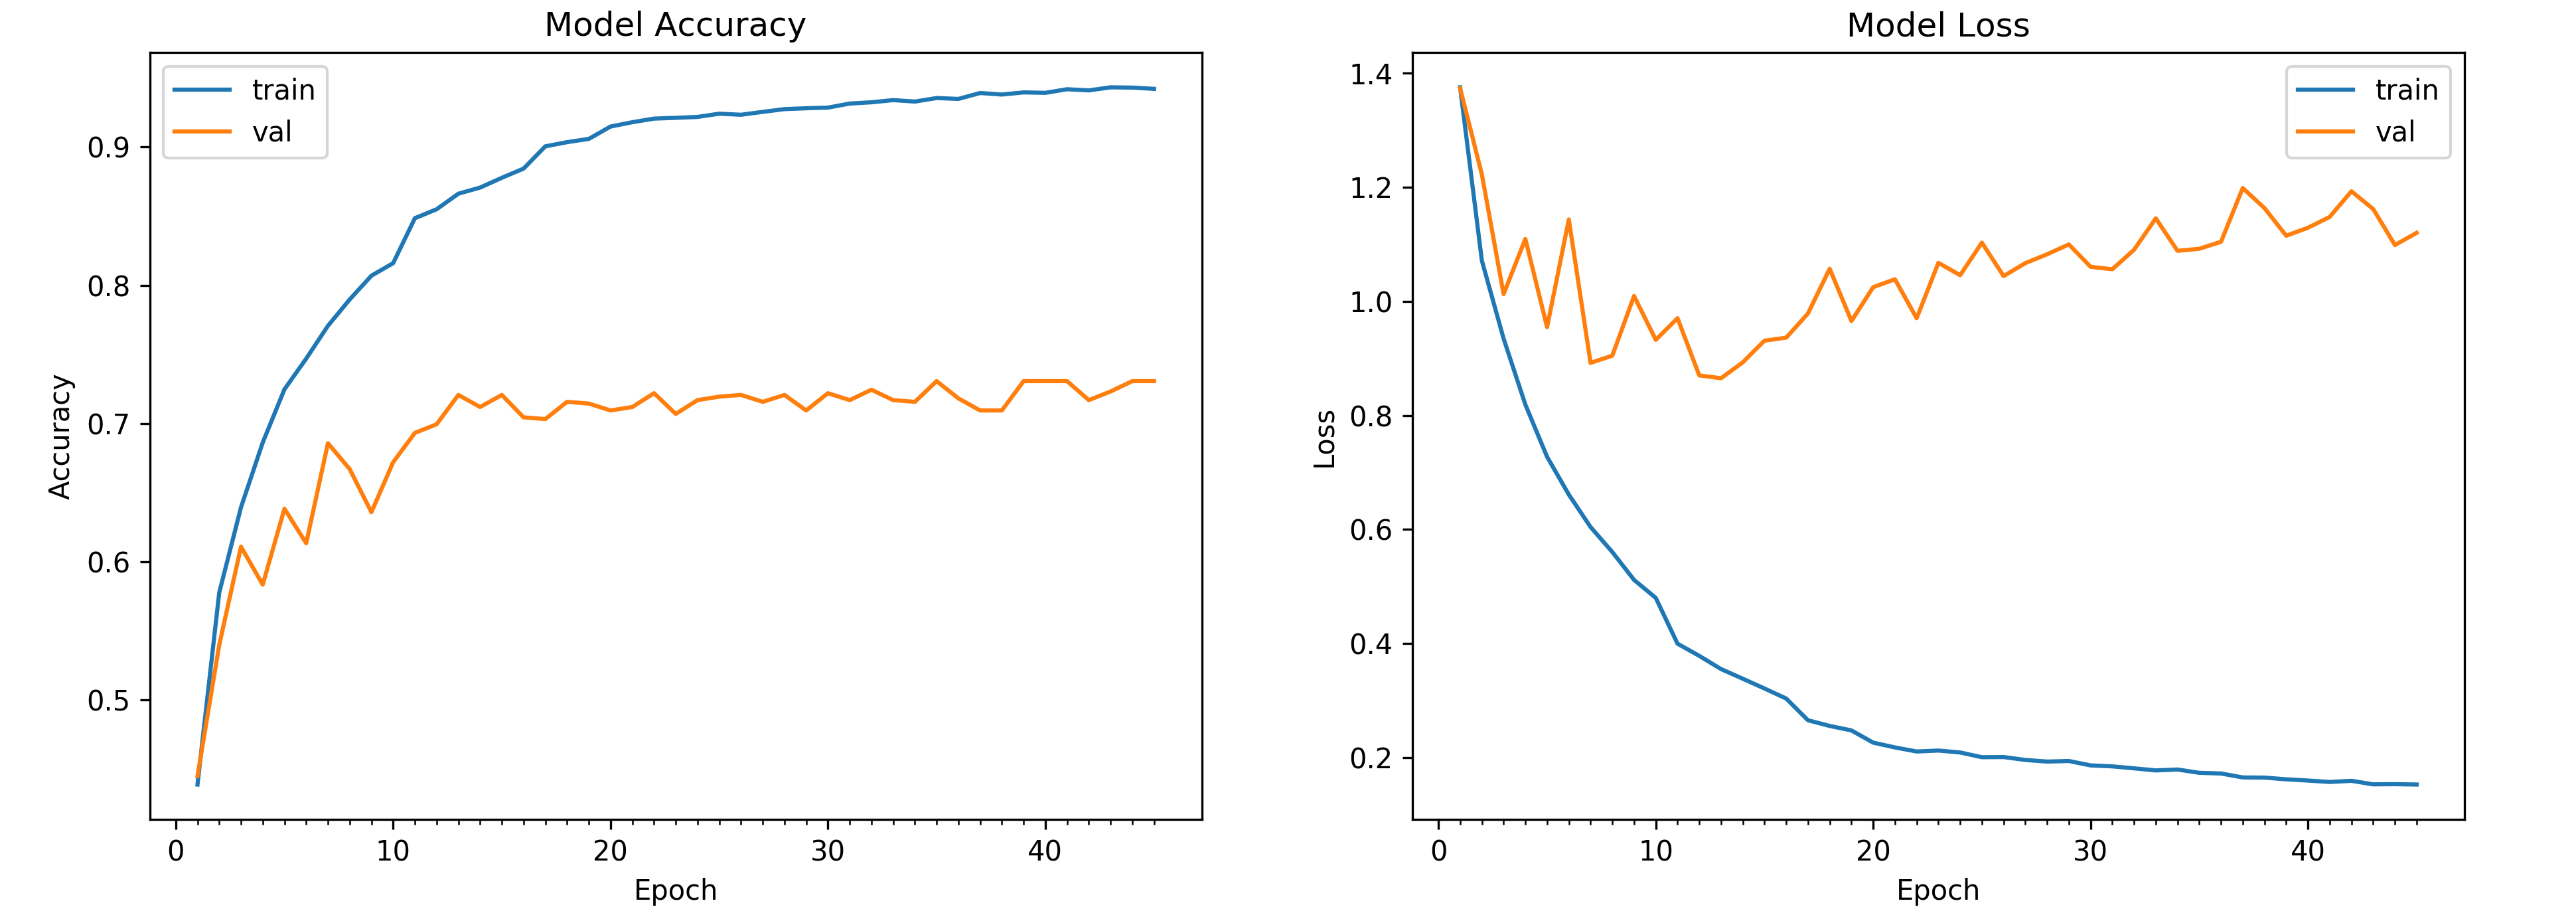
\includegraphics[width=15cm]{images/overfitting-data-aug.png}
			\caption{Plot of accuracy and loss of data augmented model}
			\label{fig:overfitting-data-aug}
		\end{figure}
		
		In Table \ref{tab:experiments_results} is possible to compare the performances on the test set of the previous three models in terms of F1 scores, macro average F1 and accuracy.
		
		\begin{table}[H]
			\centering
			\begin{tabular}{ |>{\centering\arraybackslash}p{2.5cm}|c|c|c|c|c|c|c|>{\centering\arraybackslash}p{1.5cm}|>{\centering\arraybackslash}p{2cm}| }
				\hline
				\textbf{Model} & \textbf{akiec} & \textbf{bcc} & \textbf{bkl} & \textbf{df} & \textbf{mel} & \textbf{nv} & \textbf{vasc} & \textbf{Macro average} & \textbf{Test accuracy} \\ \hline
				
				Proposed model & 0.44 & 0.55 & 0.54 & 0.17 & 0.39 & 0.90 & 0.56 & 0.51 & 0.77 \\ \hline
				Class weighting & 0.38 & 0.50 & 0.45 & 0.27 & 0.48 & 0.80 & 0.71 & 0.51 & 0.65 \\ \hline
				Oversampling & 0.46 & 0.54 & 0.53 & 0.34 & 0.47 & 0.86 & 0.75 & 0.56 & 0.72 \\ \hline
				
			\end{tabular}		
			\caption{Experiments' results}
			\label{tab:experiments_results}
		\end{table}
	
		The model trained on the oversampled training set gives better results in terms of performance measures compared to the other models, but tends to misclassifyF too much Melanomas, that are the most important class for our goal.
		So, in conclusion, even if the last model performs relatively well, we prefer to select the model with class weighting as our best model because it has performances that better meet our goal of reducing the number of misclassified skin lesions.
		
		
		
		
		
	%\section{Conclusion} \label{conclusion}
	
	Working on skin cancer classification required a lot of effort and time because it was the first time we challenged with imbalanced data. 
	Compared to the other papers our results are not that good, but researchers used transfer learning and well-known architectures to obtain their results. Instead, we tried different approaches, such as class weighting and oversampling and we have built a CNN model from scratch that was able to learn something from the challenging HAM10000 dataset. 
	We understood that with more data CNN can achieve performances that are able to outperforms expert dermatologists, and this is an important milestone in oncology. In fact, having machines capable of early detection of malignant skin cancers will allow the doctor to provide faster diagnoses and will lead to a high survival rate for this disease. Since we did not have enough time to perform other experiments we have thought to interesting future works:

	\begin{itemize}
		\item try to oversample HAM10000 with high quality images bring from hospitals' dataset or biopsy-proven datasets like DermoFit\cite{dermofit}. We tried to access to Dermofit, but it was expensive;
		\item try to apply one vs all to HAM10000. This consists in building seven classifiers, one per class, to see if model overall performances increase;
		\item try to apply other transfer learning techniques. In most of the papers, researchers tried to train a pre-trained network across all the layers. We did not have enough time and resources to try this technique;
		\item try to test the performances of our best model on other open access datasets, such as MED-NODE dataset\cite{mednode} or PH2 dataset\cite{ph2}. 	
	\end{itemize}
	
	
	% -------------------------------------------------------------------
	% Bibliography
	% -------------------------------------------------------------------

	%\bibliographystyle{unsrtnat} 
	%\bibliography{bibliography} 
	\printbibliography
	
	
	
	% -------------------------------------------------------------------
	% Appendices
	% -------------------------------------------------------------------
	
	%\begin{appendices}
		%\input{sections/appendixA.tex}
		%\input{sections/appendixB.tex}
	%\end{appendices}
	
\end{document}